\documentclass[11pt]{article}
\usepackage{amsmath,amssymb,booktabs,array, amsthm, physics, float}
\usepackage{graphicx}
\usepackage[margin=1in]{geometry}

\title{CSC311 Final Project}
\date{July 2026}

\begin{document}

\maketitle

\section*{Part A}

In the first part of the project, you will implement and apply various machine learning algorithms you studied in the course to predict students’ correctness of a given diagnostic question. Review the course notes if you don’t recall the details of each algorithm. For this part, you will only be using the primary data: \verb|train_data.csv|, \verb|sparse_matrix.npz|, \verb|valid_data.csv|, and \verb|test_data.csv|. Moreover, you may use the helper functions provided in \verb|utils.py| to load the dataset and evaluate your model. You may also use any functions from packages \verb|NumPy|, \verb|Scipy|, \verb|Pandas|, and \verb|PyTorch|. Make sure you understand the code instead of using it as a black box.

\subsection*{1. $k$-nearest neighbors.} In this problem, using the provided code at \verb|knn.py|, you will experiment with $k$-nearest neighbors (\verb|KNN|) algorithm.

The provided \verb|KNN| code performs collaborative filtering that uses other students’ answers to predict whether the specific student can correctly answer some diagnostic questions. In particular, the starter code implements user-based collaborative filtering: given a user, \verb|KNN| finds the closest user that similarly answered other questions and predicts the correctness based on the closest student’s correctness. The core underlying assumption is that if student A has the same correct and incorrect answers on other diagnostic questions as student B, A’s correctness on specific diagnostic questions matches that of student B.

\begin{enumerate}

\item[(a)] Complete a function main located at \verb|knn.py| that runs \verb|KNN| for different values of $k \in \{1,6,11,16,21,26\}$. Plot and report the accuracy on the validation data as a function of $k$

\begin{proof}[Solution.]
The validation accuracies for each value of $k$ are shown in
Table~\ref{tab:user-knn}. The corresponding validation-accuracy curve
is shown in Figure~\ref{fig:user-knn}.

\begin{center}

\begin{minipage}{0.40\textwidth}
\centering
\begin{tabular}{|c|c|}
\hline
$k$ & Validation Accuracy \\
\hline
1  & 0.6277 \\
6  & 0.6773 \\
11 & 0.6890 \\
16 & 0.6750 \\
21 & 0.6681 \\
26 & 0.6509 \\
\hline
\end{tabular}
\label{tab:user-knn}
\end{minipage}
\hfill
\begin{minipage}{0.55\textwidth}
\centering
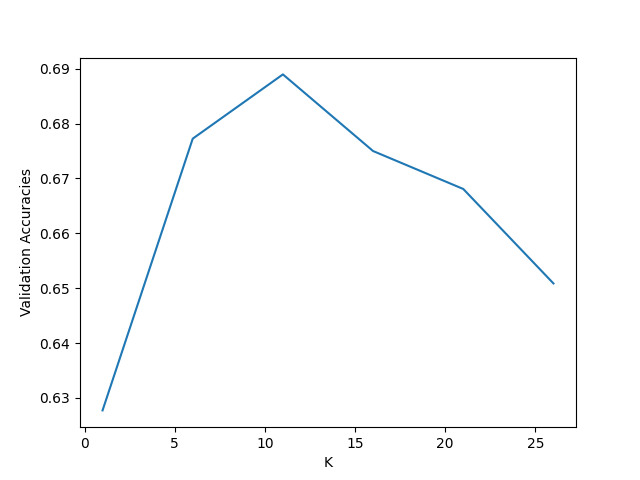
\includegraphics[width=\textwidth]{knn_validation_plot.png}
\label{fig:user-knn}
\end{minipage}

\end{center}

The validation accuracy increases until $k=11$, where it reaches its
maximum value of approximately $0.6890$. It then decreases for larger
values of $k$.
\end{proof}

\item[(b)] Choose $k^*$ that has the highest performance on validation data. Report the chosen $k^*$ and the final test accuracy.

\begin{proof}[Solution.]
    As you can see from the table above, the highest validation accuracy was from k = 11, as such our $k*$ = 11. The test accuracy from this is 0.6827547276319503.
\end{proof}

\item[(c)] Implement a function \verb|knn_impute_by_item| on the same file that performs item-based collaborative filtering instead of user-based collaborative filtering. Given a question, \verb|KNN| finds the closest question that was answered similarly, and predicts the correctness basted on the closest question’s correctness. State the underlying assumption on item-based collaborative filtering. Repeat part (a) and (b) with item-based collaborative filtering.

\begin{proof}[Solution.]
The assumption for this is that questions that are answered similarly by
the same students are very similar. Therefore, we can use a similar
question that a student answered to predict whether the student answered
another question correctly or incorrectly.

The validation accuracies obtained using item-based collaborative
filtering are shown below.

\begin{center}

\begin{minipage}{0.40\textwidth}
\centering
\begin{tabular}{|c|c|}
\hline
$k$ & Validation Accuracy \\
\hline
1  & 0.6178 \\
6  & 0.6605 \\
11 & 0.6804 \\
16 & 0.6868 \\
21 & 0.6898 \\
26 & 0.6885 \\
\hline
\end{tabular}
\label{tab:item-knn}
\end{minipage}
\hfill
\begin{minipage}{0.55\textwidth}
\centering
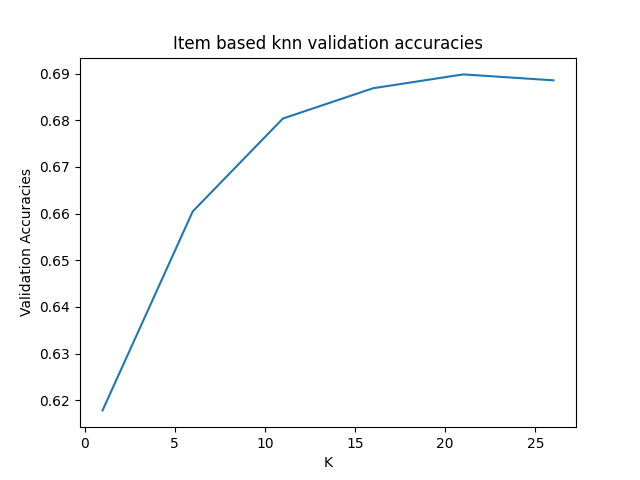
\includegraphics[width=\textwidth]{knn_validation_items_plot.png}
\label{fig:item-knn}
\end{minipage}

\end{center}

The validation accuracy generally increases as $k$ increases. The highest
validation accuracy is approximately $0.6898$, obtained at $k=21$.
Therefore, we select
\[
k^* = 21.
\]

Using $k^*=21$, the final test accuracy is \textbf{0.6810612475303415}.
\end{proof}

\item[(d)] Compare the test performance between user- and item- based collaborative filtering. State which method performs better.

\begin{proof}[Solution.]
    They perform very similarly, both have test accuracy of about 0.68. However, the user based collaborative filtering performs slightly better than the item based one with a test accuracy of about 0.6828 instead of 0.6811.
\end{proof}

\item[(e)] List at least two potential limitations of \verb|KNN| for the task you are given.

\begin{proof}[Solution.]
    One limitation of KNN is that it only uses students response patterns and does not directly consider important question characteristics such as the topic of the question, maybe a student is better at some topics than others. Therefore, questions with similar answer patterns may be treated as similar even when they cover different topics. 

A second limitation is that the response matrix is sparse. Many pairs of students or questions have only a small number of common answers, so the calculated distances between them may not accurately represent their similarity. 

KNN also has difficulty making predictions for new students or questions with very few recorded responses. 

The curse of dimensionality also applied here since we have a lot of questions. 
\end{proof}

\end{enumerate}

\subsection*{2. Item Response Theory.} In this problem, you will implement an Item-Response Theory (IRT) model to predict students’ correctness to diagnostic questions.

The IRT assigns each student an ability value and each question a difficulty value to formulate a probability distribution. In the one-parameter IRT model, $\beta_j$ represents the difficulty of the question $j$, and $\theta_i$ that represents the $i$-th students ability. Then, the probability that the question $j$ is correctly answered by student $i$ is formulated as:

\[
p(c_{ij} = 1 \mid \theta_i, \beta_j) = \frac{\exp(\theta_i - \beta_j)}{1 + \exp(\theta_i - \beta_j)}
\]

We provide the starter code in \verb|item_response.py|.

\begin{enumerate}

\item[(a)] Derive the log-likelihood $\log p(\mathbf{C}\mid\boldsymbol{\theta},\boldsymbol{\beta})$ for all students and questions. Here $\mathbf{C}$ is the sparse matrix. Also, show the derivative of the log-likelihood with respect to $\theta_i$ and $\beta_j$ (Hint: recall the derivative of the logistic model with respect to the parameters).

\begin{proof}[Solution.]
    Let $\mathcal{O}$ be the set of $(i, j)$ pairs that have been observed, that is their entry in the sparse matrix exists.

    Note that for a single outcome, we will use the Bernoulli distribution to get the probability of the likelihood as,

    \begin{align*}
        p(c_{ij} \mid \theta_i, \beta_j) &= (\frac{\exp(\theta_i - \beta_j)}{1 + \exp(\theta_i - \beta_j)})^{c_{ij}}(1 - \frac{\exp(\theta_i - \beta_j)}{1 + \exp(\theta_i - \beta_j)})^{1 - c_{ij}} \\
        &= (\frac{\exp(\theta_i - \beta_j)}{1 + \exp(\theta_i - \beta_j)})^{c_{ij}}(\frac{1}{1 + \exp(\theta_i - \beta_j)})^{1 - c_{ij}}
    \end{align*}

    We get the log-likelihood as 

    \begin{align*}
        \log(\mathbf{C} \mid \boldsymbol{\theta}, \boldsymbol{\beta}) &= \sum_{(i, j) \in \mathcal{O}}\log(p(c\mid \theta_i, \beta_j)) \\
        &= \sum_{(i, j) \in \mathcal{O}}\log((\frac{\exp(\theta_i - \beta_j)}{1 + \exp(\theta_i - \beta_j)}^{c_{ij}})(\frac{1}{1 + \exp(\theta_i - \beta_j)})^{1 - c_{ij}}) \\
        &= \sum_{(i, j) \in \mathcal{O}} c_{ij}(\theta_i - \beta_j - \log(1+\exp(\theta_i - \beta_j)))-(1-c_{ij})\log(1 + \exp(\theta_i - \beta_j)) \\
        &= \sum_{(i, j) \in \mathcal{O}}c_{ij}(\theta_i - \beta_j) - \log(1 + \exp(\theta_i - \beta_j))
    \end{align*}

    We then find the derivative of the log likelihood with respect to $\theta_i$ first. Let $\log(\mathbf{C} \mid \boldsymbol{\theta}, \boldsymbol{\beta}) = f$ for notation simplicity.

    Then, 

    \begin{align*}
    \frac{df}{d\theta_i} &= \frac{d}{d\theta_i}[\sum_{(i, j) \in \mathcal{O}} c_{ij}(\theta_i - \beta_j) - \log(1 + \exp(\theta_i - \beta_j))] \\
    &= \sum_{i : (i, j) \in \mathcal{O}}c_{ij} - \frac{\exp(\theta_i - \beta_j)}{1 + \exp(\theta_i - \beta_j)} \\
    &= \sum_{i : (i, j) \in \mathcal{O}}c_{ij} - \sigma(\theta_i - \beta_j)
    \end{align*}

    where note that we identify the following expression $\frac{\exp(x)}{1 +\exp(x)} = \sigma(x)$ is the sigmoid function, and for our indexing of the sum, $i: (i, j) \in \mathcal{O}$ refers to all entries $(i, j) \in \mathcal{O}$ that exist in the sparse matrix, given a fixed $i$. We similarly get the derivative of the log likelihood with respect to $\beta_j$ as,

    \begin{align*}
    \frac{df}{d\beta_j} &= \frac{d}{d\beta_j}[\sum_{(i, j) \in \mathcal{O}} c_{ij}(\theta_i - \beta_j) - \log(1 + \exp(\theta_i - \beta_j))] \\
    &= \sum_{j : (i, j) \in \mathcal{O}}\frac{\exp(\theta_i - \beta_j)}{1 + \exp(\theta_i - \beta_j)} - c_{ij} \\
    &= \sum_{j : (i, j) \in \mathcal{O}}\sigma(\theta_i - \beta_j) - c_{ij}
    \end{align*}
\end{proof}

\item[(b)] Implement missing functions in \verb|item_response.py| that performs alternating gradient descent on $\boldsymbol{\theta}$ and $\boldsymbol{\beta}$ to maximize the log-likelihood. Report the hyperparameters you selected. With your chosen hyperparameters, report the training curve that shows the training and validation log-likelihoods as a function of iteration.

\begin{proof}[Solution.]
    Refer to \verb|item_response.py| for the implemented code.
    The learning rate we used was $0.01$ and the number of iterations was chosen to be $50$. The training curve showing the training and validation log-likelihoods as a function of iterations is given below:

    \begin{center}
    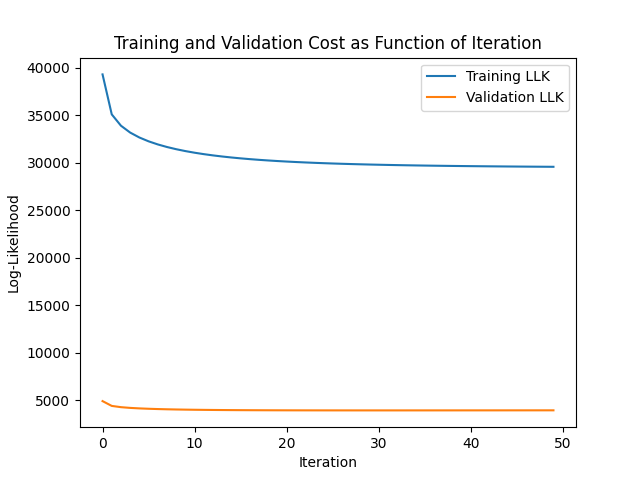
\includegraphics[width=0.8\textwidth]{q2b.png}
    \end{center}
\end{proof}

\item[(c)] With the implemented code, report the final validation and test accuracies.

\begin{proof}[Solution.]
    The final validation accuracy was 0.7060 and the test accuracy was 0.7070. The training accuracy was also 0.7395.
\end{proof}

\item[(d)] Select three questions $j_1,j_2,$ and $j_3$. Using the trained $\boldsymbol{\theta}$ and $\boldsymbol{\beta}$, plot three curves on the same plot that shows the probability of the correct response $p(c_{ij} = 1)$ as a function of $\boldsymbol{\theta}$ given a question $j$. Comment on the shape of the curves and briefly describe what these curves represent.

\begin{proof}[Solution.]
    We chose questions $j_1 = 0, j_2 = 100, j_3 = 500$, and plotted the probability $p(c_{ij} = 1)$ as a function of $\boldsymbol{\theta}$ given question $j$ shown below:

    \begin{center}
        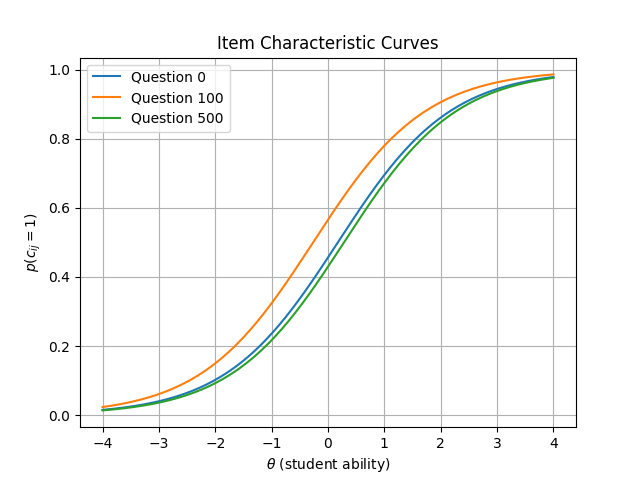
\includegraphics[width=0.8\textwidth]{q2d.png}
    \end{center}

    As expected, we get the following sigmoid curves since our probability is defined by the sigmoid function. The following curves represent how the probability of getting a correct answer depends on a student's ability, with higher student ability logistically increasing the probability of getting the answer correct.
    
    We see that question 100 is shifted to the left more than the curves representing question 0 and 500, suggesting that question 100 is easier than questions 0 and 500 as it requires less student ability for higher probability of correct answers. Question 500 seems to be the hardest out of the three as it is shifted to the right the most, meaning it requires more student ability to get higher probability of a correct answer.
    
\end{proof}

\end{enumerate}

\subsection*{3. Neural Networks} In this problem, you will implement neural networks to predict students’ correctness on a diagnostic question. Specifically, you will design an autoencoder model. Given a user $\mathbf{v} \in \mathbb{R}^{N_{questions}}$ from a set of users $\mathcal{S}$, our objective is:

\[
    \min_{\boldsymbol{\theta}}\sum_{\mathbf{v} \in \mathcal{S}}||\mathbf{v} - f(\mathbf{v}; \boldsymbol{\theta})||_2^2
\]

where $f$ is the reconstruction of the input $\mathbf{v}$. The network computes the following function:

\[
    f(\mathbf{v};\boldsymbol{\theta}) = h(\mathbf{W}^{(2)}g(\mathbf{W}^{(1)}\mathbf{v} + \mathbf{b}^{(1)}) + \mathbf{b^{(2)}}) \in \mathbb{R}^{N_{questions}}
\]

for some activation functions $h$ and $g$. In this question, you will be using sigmoid activation functions for both. Here, $\mathbf{W}^{(1)} \in \mathbb{R}^{k \times N_{questions}}$ and $\mathbb{W}^{(2)} \in \mathbb{R}^{N_{questions} \times k}$, where $k \in N$ is the latent dimension. We provide the starter code written in \verb|PyTorch| at \verb|neural_network.py|.

\begin{enumerate}

\item[(a)] Describe at least three differences between ALS and neural networks.

\begin{proof}[Solution.]
    The major difference between ALS and neural networks is that neural networks allow for more complex non-linear relationships to be captured,
    since ALS is a set of linear regression subproblems, but neural networks allow for non-linear activation functions to be used, which allows more expressiveness in our model.

    Another difference is that ALS is utilized for specifically matrix factorization problems, whereas neural networks can be used for much more different tasks such as image classification, natural language processing, or regression problems.

    Finally, the method of optimization for ALS and neural networks differ because ALS works on solving for one set of latent factors while keeping the other set fixed, and then working on the other set while keeping the ones we just worked on fixed, and repeating this process until convergence, determined by a hyperparameter stating the number of iterations usually.
    It is important to note that ALS will always have a closed form solution for each update we do on the set of latent factors, whereas neural networks may not. Therefore, neural networks usually use gradient-based optimizations such as backpropagation with stochastic gradient descent.
\end{proof}

\item[(b)] Implement a class \verb|AutoEncoder| that performs a forward pass of the autoencoder following the instructions in the docstring.

\begin{proof}[Solution.]
    See the following code in \verb|neural_networks.py| to see the implementation of the class \verb|AutoEncoder|.
\end{proof}

\item[(c)] Train the autoencoder using latent dimensions of $k \in \{10,50,100,200,500\}$. Also, tune optimization hyperparameters such as learning rate and number of iterations. Select $k^*$ that has the highest validation accuracy.

\begin{proof}[Solution.]
We found that $k^* = 50$ with learning rate $\alpha = 0.01$ and $\#\text{epoch} = 40$ achieved the highest validation score of about 0.69.
\end{proof}

\item[(d)] With your chosen $k^*$, plot and report how the training and validation objectives changes as a function of epoch. Also, report the final test accuracy.

\begin{proof}[Solution.]

    The training and validation objectives were plotted as a function of epoch below:

    \begin{center}
        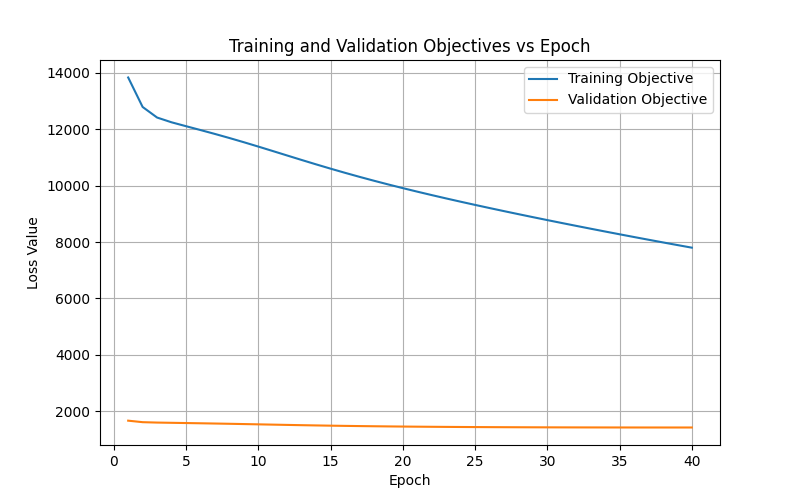
\includegraphics[width=0.8\textwidth]{q3d_without_reg.png}
    \end{center}

    The final test accuracy acquired by our model was 0.6887.

\end{proof}

\item[(e)] Modify a function train so that the objective adds the $L_2$ regularization. The objective is as follows:

\[
    \min_{\boldsymbol{\theta}}\sum_{\mathbf{v} \in \mathcal{S}} ||\mathbf{v} - f(\mathbf{v; \boldsymbol{\theta}})||_2^2 + \frac{\lambda}{2}(||\mathbf{W}^{(1)}||_F^2 + ||\mathbf{W}^{(2)}||_F^2)
\]

You may use a method \verb|get_weight_norm| to obtain the regularization term. Using the $k$ and other hyperparameters selected from part (d), tune the regularization penalty $\lambda \in \{0.001,0.01,0.1,1\}$. With your chosen $\lambda$, report the final validation and test accuracy. Does your model perform better with the regularization penalty?

\begin{proof}[Solution.]
    With the same $k* = 50$ and other parameters from part (d), we chose $\lambda^* = 0.01$, which performs just slightly worse than the base model with no regularization penalty, but it reaches the optimal value much faster. The final validation accuracy was 0.679 and the final test accuracy was 0.677.

    The validation and training objectives are once again plotted below as a function of epoch, and it shows a more smoothed curve which is to be expected due to the regularization penalty.

    \begin{center}
        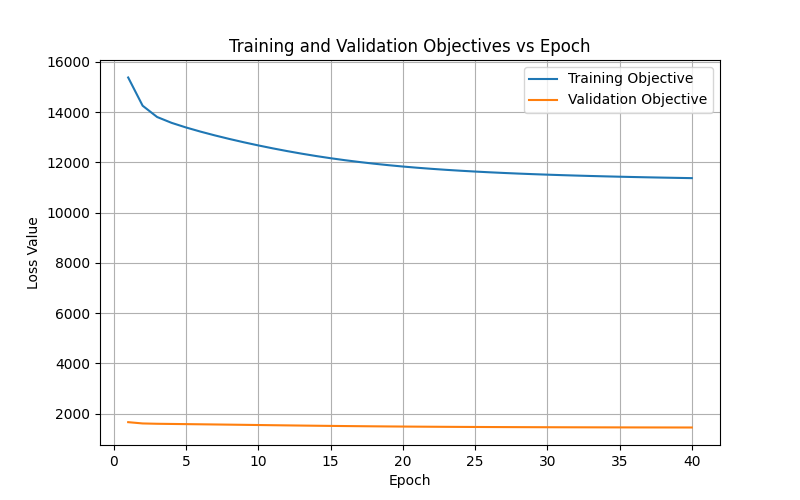
\includegraphics[width=0.8\textwidth]{q3e.png}
    \end{center}
\end{proof}

\end{enumerate}

\subsection*{4. Ensemble} In this problem, you will be implementing bagging ensemble to improve the stability and accuracy of your base models. Select and train 3 base models with bootstrapping the training set. You may use the same or different base models. Your implementation should be completed in \verb|ensemble.py|. To predict the correctness, generate 3 predictions by using the base model and average the predicted correctness. Report the final validation and test accuracy. Explain the ensemble process you implemented. Do you obtain better performance using the ensemble? Why or why not?

\begin{proof}[Solution.]
    I tried 2 different ensembles, one with 3 IRT base models with the same optimal hyper parameters as found in question 2 and one with 2 Neural Networks and 1 IRT model in which I tuned the hyper parameters with the validation set. I will be reporting on the second one. In this ensemble I made a dictionary data set by selecting random rows with replacement in the csv for the IRT model. I then generated 2 lists of randomly selected user ids with replacement to train the autoencoders on, the lists were the same size as the number of total users. Then after getting predictions for the IRT the the 2 NNs, i took the final prediction to be the mean of hte 3 predictions. For this ensemble I found the optimal hyper parameters to be k=50, irt learning rate=0.02, irt iterations=50, neural network learning rate=0.03, neural network epochs=20, neural network lambda=0.01. I used the same hyper parameters for both the neural networks. I found that the ensemble had a validation accuracy of 0.69249 and a final test accuracy of 0.6915. This is higher than the final test accuracy of the single neural network but lower than the final test accuracy of the single IRT model. I got a worse performance than just using a single IRT model as the single IRT model had a higher accuracy than the single neural network model, as such, the 2 neural networks are just lowering the accuracy as they are less fit for the task than the IRT. Furthermore, when I also tried using an ensemble of 3 IRT models, the result was a worse final test accuracy than the single IRT model. Which led me to believe that maybe using an ensemble with bagging in general may be worse than using a single model. I think this could be because bagging in general is most useful for unstable models with high variance in their predictions. IRT is a stable model so using a bagging ensemble just makes 3 models train on less distinct data sets and I think this ultimately under fits the data thus yielding a lower final test accuracy.
\end{proof}

\section*{Part B}

We will focus on the Item Response Theory from part A, as it showed the highest result and is a very optimized algorithm that finds the optimum parameter values relatively quickly. We will improve upon it for part B using the given \verb|question_meta.csv| first. The updated code will be located in \verb|irt_test.py|.

Let's introduce a sparse matrix $\boldsymbol{\delta} \in \mathbb{R}^{N_{\text{students}} \times N_{\text{subjects}}}$ of parameters that $\delta_{i,k(j)}$ where $i$ refers to a student, and $k(j)$ is a representative subject assigned to question $j$. \verb|subject_meta.csv| gives us the hierarchical subject that each question falls under, so let's try to subdivide our data into certain subjects in order to introduce information based on the subject a question falls under. We want to essentially learn about the ability for students to handle certain subjects compared to others in order to hopefully improve our predictions further. $\delta_{i, k(j)}$ will represent the deviation of student $i$'s ability on subject $k(j)$ from their overall ability $\theta_i$, acting as a sort of bias term.

The new probability that the question $j$ of subject $k$ is correctly answered by student $i$ is given by:

\[
p(c_{ij} = 1 \mid \theta_i, \beta_j, \delta_{i, k(j)})
= 
\frac{\exp(\theta_i + \delta_{i,k(j)} - \beta_j)}{1+\exp(\theta_i + \delta_{i,k(j)} - \beta_j)}
\]

The log likelihood remains fairly similar to the original IRT, where $f = \log(\mathbf{C} \mid \boldsymbol{\theta}, \boldsymbol{\beta}, \boldsymbol{\delta})$. Let's also add a Frobenius $L_2$ regularization term just on the $\boldsymbol{\delta}$ parameter, $\frac{\lambda}{2}||\boldsymbol{\delta}||^2_2$, then the new gradients to use during the optimization will be:

\begin{align*}
\frac{df}{d\theta_i} &= \sum_{(i, j) \in \mathcal{O}} c_{i,j} - \sigma(\theta_i + \delta_{i, k(j)} - \beta_{j}) \\
\frac{df}{d\beta_{j}} &= \sum_{(i, j) \in \mathcal{O}}{\sigma(\theta_i + \delta_{i, k(j)} - \beta_{j})} - c_{i,j} \\
\frac{df}{d\delta_{i, k(j)}} &= \sum_{(i, j) \in \mathcal{O}}{(c_{i, j}-\sigma(\theta_i + \delta_{i, k(j)} - \beta_{j}))} -\lambda\delta_{i, j(k)} 
\end{align*}

The following code is also update from the base model in the new file \verb|irt_test.py|. Since the questions are divided into subjects hierarchically, our subject representative mapping will acquire the subject id of question $j$ at depth $d$, that is $k:Q \times D \to S$, where $Q \subseteq \mathbb{N}$ is the set of question ids, and $D \subseteq \mathbb{N}$ is the set of valid depths, and $S \subseteq \mathbb{N}$ is the set of subject ids. In the csv file, a question id has an associated subject id list, for example question id 45 may have subject id $[0, 4, 14, 239, 87]$, so then $k(45, 2) = 4$ gets the subject id of question id $45$ at depth $2$ which is $4$ in our case. In the csv file, all questions have root subject id $0$, denoted as Maths in \verb|subject_meta.csv|. 

We will start with a depth of $2$ to analyze the behaviour of our model. We will also keep track of the most common subject, meaning the subject that most questions fall under, as well as the rarest subject, meaning the subject that is not categorized under most questions. This stratification will become useful to analyze how our sparse matrix may affect the accuracy within each subject themselves, as opposed to just computing the overall accuracy of the dataset. Below is a table showcasing the configuration of the model we used, the lambda value used, the overall training, validation and accuracy scores of the whole dataset, as well as the scores for each strata. We can keep the same hyperparameter from our base IRT of $\alpha = 0.01$ and number of iterations at $50$ for now, as we sweep through $\lambda$ values. Keep in mind that the most common subject were associated to 3515 examples, whereas the least common subject was only associated to 28 examples for the test set. In the training set, the most common subject had 56180 examples, and the least common subject had 508 examples.

\begin{table}[ht]
\centering
\caption{Performance of the baseline IRT model and the subject-$\delta$ IRT model under different regularization strengths. Test accuracies for common and rare subjects are computed over 3515 and 28 test examples, respectively.}
\label{tab:lambda_sweep}
\begin{tabular}{lcccccc}
\hline
Model & $\lambda$ & Train & Validation & Test & Test (Common) & Test (Rare) \\
\hline
Baseline IRT & -- & 0.7395 & 0.7060 & 0.7070 & -- & -- \\
\hline
Subject-$\delta$ & 0.00  & 0.7478 & 0.7058 & \textbf{0.7099} & \textbf{0.7104} & 0.6429 \\
Subject-$\delta$ & 0.01  & 0.7478 & 0.7056 & \textbf{0.7099} & \textbf{0.7104} & 0.6429 \\
Subject-$\delta$ & 0.05  & 0.7477 & 0.7058 & 0.7096 & 0.7101 & 0.6429 \\
Subject-$\delta$ & 0.20  & 0.7477 & 0.7059 & 0.7093 & 0.7098 & 0.6429 \\
Subject-$\delta$ & 1.00  & 0.7475 & 0.7058 & 0.7084 & 0.7090 & 0.6429 \\
Subject-$\delta$ & 5.00  & 0.7458 & \textbf{0.7094} & \textbf{0.7099} & 0.7101 & \textbf{0.6786} \\
Subject-$\delta$ & 10.00 & 0.7446 & 0.7075 & 0.7090 & 0.7098 & 0.6071 \\
Subject-$\delta$ & 20.00 & 0.7434 & 0.7069 & 0.7087 & 0.7092 & 0.6429 \\
Subject-$\delta$ & 50.00 & 0.7418 & 0.7069 & 0.7084 & 0.7090 & 0.6429 \\
\hline
\end{tabular}
\end{table}

We see that from table 1, our new IRT model with the subject $\boldsymbol{\delta}$ matrix is performs slightly better than our base IRT even with no regularization due to additional information provided by the subject associated with each question. However, notice that as our $\lambda$ value increases, at specifically $\lambda = 5$, we see that the test accuracy for the rare subject strata increases a considerable amount, but since there is very few rare-subject examples, this is not a meaningful result as this essentially means we gained one additional correct prediction from say $\lambda = 0$. The common subjects still dominate our dataset so the rare subject accuracy being low will not contribute much to our overall accuracy. 

Now, let's try to perform a depth sweep from a depth of $1$ to $9$, as the highest depth of question-subject hierarchy I saw in the metadata csv was $9$. We should expect to see that the accuracy for rare subjects go up as the stratification of the data will become more distributed, as there will be more subjects that each question lie under rather than a few select subjects. This in turn should also cause our model to learn the training data better, potentially adding some issues involving overfitting for higher depths. A table is given below, with lambda replaced by depth, and two additional columns to give us the number of test examples associated to the most common subject and least common subject at depth $d$. For this, keep $\lambda = 5$ fixed.

\begin{table}[H]
\centering
\small
\setlength{\tabcolsep}{4pt}
\begin{tabular}{c|c|ccc|cc|cc}
\hline
\textbf{Model} & \textbf{Depth}
& \textbf{Train} & \textbf{Val} & \textbf{Test}
& \textbf{Test Common} & \textbf{$N_c$}
& \textbf{Test Rare} & \textbf{$N_r$} \\
\hline
IRT & --
& 0.7395 & 0.7060 & 0.7070
& -- & --
& -- & -- \\

Subject-$\delta$ IRT & 1
& 0.7458 & \textbf{0.7094} & \textbf{0.7099}
& 0.7101 & 3515
& 0.6786 & 28 \\

Subject-$\delta$ IRT & 2
& 0.7588 & 0.7060 & 0.7087
& 0.7099 & 2003
& 0.7071 & 1540 \\

Subject-$\delta$ IRT & 3
& 0.7617 & 0.7077 & 0.7056
& 0.6986 & 866
& 0.7079 & 2677 \\

Subject-$\delta$ IRT & 4
& 0.7612 & 0.7076 & 0.7059
& 0.6995 & 882
& 0.7080 & 2661 \\

Subject-$\delta$ IRT & 5
& 0.7612 & 0.7075 & 0.7067
& 0.7033 & 947
& 0.7080 & 2596 \\

Subject-$\delta$ IRT & 6
& 0.7616 & 0.7067 & 0.7067
& 0.7096 & 878
& 0.7058 & 2665 \\

Subject-$\delta$ IRT & 7
& 0.7615 & 0.7066 & 0.7067
& 0.7080 & 870
& 0.7063 & 2673 \\

Subject-$\delta$ IRT & 8
& 0.7614 & 0.7069 & 0.7067
& 0.7086 & 875
& 0.7061 & 2668 \\

Subject-$\delta$ IRT & 9
& 0.7614 & 0.7069 & 0.7067
& 0.7086 & 875
& 0.7061 & 2668 \\

\hline
\end{tabular}
\caption{Performance comparison between baseline IRT and Subject-$\delta$ IRT models across different subject hierarchy depths. $N_c$ and $N_r$ denote the number of common and rare subject examples in the test set, respectively.}
\label{tab:subject_delta_results}
\end{table}

As the hierarchy depth increases, the model is provided with increasingly fine-grained subject categories, resulting in more subject-specific $\delta$ parameters. Although this allows the model to better fit the training data, the additional parameters are estimated from fewer observations per subject and are therefore more susceptible to noise. This is reflected by the gradual increase in training accuracy from 0.7458 at depth 1 to approximately 0.7615 for depths 3--9, while the test accuracy decreases or remains close to the baseline. Therefore, finer subject hierarchies appear to capture subject-specific patterns that do not generalize well to unseen data.

The common and rare subject analysis further highlights this tradeoff. At depth 1, the model achieves a higher accuracy on common subjects (0.7101), but performs poorly on rare subjects (0.6786), although the rare category contains only 28 test examples. For deeper hierarchies, the number of rare-subject examples increases substantially, producing more reliable estimates of rare-subject performance. Despite this, the rare-subject accuracy remains similar across depths (approximately 0.706--0.708), indicating that increasing subject granularity does not provide a significant advantage for handling less frequently observed subjects.

Overall, the results indicate that a shallow subject hierarchy provides the best balance between model flexibility and generalization. The depth-1 Subject-$\delta$ IRT model improves over the baseline by incorporating subject-level student variation while avoiding the overfitting introduced by more detailed subject representations.

Repeating our fine tuning of regularization can improve our higher depth models, as an example, I ran with depth 6 and $\lambda = 20$ and we acquired the following result in table 3.

\begin{table}[h]
\centering
\small
\setlength{\tabcolsep}{6pt}
\begin{tabular}{c|c|ccc|cc|cc}
\hline
\textbf{Model} & \textbf{Depth} 
& \textbf{Train} & \textbf{Val} & \textbf{Test}
& \textbf{Test Common} & $\mathbf{N_c}$
& \textbf{Test Rare} & $\mathbf{N_r}$ \\
\hline
Subject-$\delta$ IRT ($\lambda=20$) & 6
& 0.7460 & 0.7062 & 0.7070
& \textbf{0.7130} & 878
& 0.7051 & 2665 \\
\hline
\end{tabular}
\caption{Performance of the Subject-$\delta$ IRT model using hierarchy depth 6 and regularization strength $\lambda=20$.}
\label{tab:lambda20_depth6}
\end{table}

As we see, the regularization helps with the overfitting issue considerably as our training accuracy lowers, but this gives similar results as using the base IRT in terms of the test accuracy. More importantly however, our common-subject test examples are predicted much better, but our rare-subject test accuracy went slightly lower due to the loss of subject-specific adaptation. This tradeoff remains beneficial, as the model achieves improved performance on well-represented subjects while reducing the variance introduced by higher-depth subject representations.

The last real fine tuning we gathered from this subject $\boldsymbol{\delta}$ model was to consider utilizing multiple depths of subjects for a question, so that we could see how all subjects that a question is related to influences the prediction for a model. This means that the mapping function will now return a list of subjects associated to a question, so define $k_d : Q \to S_d$ where $Q$ is the set of question ids, and $S_d$ is the set of subjects at hierarchy depth $d$. If a question $q$ does not have a subject at depth $d'$, simply $k_{d'}(q) = 0$. Our new entry in the matrices will be $\Delta_{i,j} = \sum_{n=1}^{d}{\Delta_{i,k_n(j)}}$ (note this is not a recursive definition, it just uses the values in the current matrix), and our matrix $\boldsymbol{\Delta}$ still has the same dimensions as we previously described. Note, we skip the 0th depth since all questions hold the same root subject so this information is meaningless to any information gain. The following results using this method is found using $\lambda = 20$, since this introduces much more parameters within our $\boldsymbol{\Delta}$ matrix, so we need to account for the overfitting by raising our regularization constant.

\begin{table}[H]
\centering
\small
\setlength{\tabcolsep}{4pt}
\begin{tabular}{c|c|ccc|cc|cc}
\hline
\textbf{Model} & \textbf{Max Depth}
& \textbf{Train} & \textbf{Val} & \textbf{Test}
& \textbf{Test Common} & \textbf{$N_c$}
& \textbf{Test Rare} & \textbf{$N_r$} \\
\hline
IRT & --
& 0.7395 & 0.7060 & 0.7070
& -- & --
& -- & -- \\

Subject-$\Delta$ IRT & 1
& 0.7434 & 0.7069 & 0.7087
& 0.7092 & 3515
& 0.6429 & 28 \\

Subject-$\Delta$ IRT & 2
& 0.7493 & 0.7079 & 0.7099
& 0.7104 & 3515
& 0.7095 & 1532 \\

Subject-$\Delta$ IRT & 3
& 0.7544 & 0.7069 & \textbf{0.7104}
& 0.7112 & 3515
& 0.7110 & 2938 \\

Subject-$\Delta$ IRT & 4
& 0.7549 & 0.7070 & \textbf{0.7104}
& 0.7112 & 3515
& \textbf{0.7113} & 2989 \\

Subject-$\Delta$ IRT & 5
& 0.7549 & 0.7072 & 0.7087
& 0.7095 & 3515
& 0.7100 & 3014 \\

Subject-$\Delta$ IRT & 6
& 0.7550 & 0.7070 & 0.7093
& 0.7101 & 3515
& 0.7104 & 3014 \\

Subject-$\Delta$ IRT & 7
& 0.7551 & 0.7075 & 0.7093
& 0.7101 & 3515
& 0.7104 & 3014 \\

Subject-$\Delta$ IRT & 8
& 0.7552 & \textbf{0.7076} & 0.7096
& 0.7104 & 3515
& 0.7107 & 3014 \\

Subject-$\Delta$ IRT & 9
& 0.7552 & \textbf{0.7076} & 0.7096
& 0.7104 & 3515
& 0.7107 & 3014 \\

\hline
\end{tabular}
\caption{Performance comparison between the baseline IRT model and the hierarchical Subject-$\delta$ IRT model, where a maximum depth of $d$ indicates that all subject ancestors from depths $1$ through $d$ are included. $N_c$ and $N_r$ denote the number of common and rare test examples, respectively.}
\label{tab:hierarchical_subject_delta_results}
\end{table}

From table 4, we see that indeed providing more subject information to each question gives better results, much better results than the base IRT, but only provides a small improvement over using just 1 representative subject per question.

The last major architectural change we want to attempt is to combine IRT for handling the main optimization, but use autoencoders to reduce the dimensionality of our $\boldsymbol{\Delta}$ matrix and consider utilizing a user latent/subject embedding pair to handle the matrix entries. The updated code will be provided in \verb|irt_autoencoder.py|.

Let $k \in \mathbb{N}$ be the latent dimension. A user $i$ has a latent representation $z_i \in \mathbb{R}^k$ and each subject $s$ has an embedding $e_s \in \mathbb{R}^k$ so that we can approximately calculate the subject effect as $\Delta_{ij} = \sum_{n=1}^{d}z_i^Te_{k_{n}(j)}$. The autoencoder will essentially pretrain the subject embedding and latent user space and the IRT model will fine tune them further to give better predictions. 
Then our new likelihood model will become

\[
p(c_{ij} = 1 | \theta_i, \beta_j, z_i, e_s) = \frac{\exp(\theta_i + \sum_{n=1}^{d}{z_i^T}e_{k_n(j)} - \beta_j) }{1 + \exp(\theta_i + \sum_{n=1}^{d}{z_i^T}e_{k_n(j)} - \beta_j)}
\]

The gradient of the log likelihood with respect to each parameter is given below:

\begin{align*}
\frac{df}{d\theta_i} &= \sum_{(i, j) \in \mathcal{O}} c_{i,j} - \sigma(\theta_i + \sum_{n=1}^{d}{z_i^T}e_{k_n(j)} - \beta_{j}) \\
\frac{df}{d\beta_{j}} &= \sum_{(i, j) \in \mathcal{O}}{\sigma(\theta_i + \sum_{n=1}^d{z_i^T}e_{k_n(j)} - \beta_{j})} - c_{i,j} \\
\frac{df}{dz_i} &=\sum_{(i,j)\in\mathcal{O}}\left(c_{i,j}-\sigma\left(\theta_i+\sum_{n=1}^{d} z_i^T e_{k_n(j)}-\beta_j\right)\right)\left(\sum_{n=1}^{d} e_{k_n(j)}\right) \\
\frac{df}{de_s}&=\sum_{\substack{(i,j)\in\mathcal{O}\\s\in\{k_1(j),...,k_d(j)\}}}\left(c_{i,j}-\sigma\left(\theta_i+
\sum_{n=1}^{d} z_i^T e_{k_n(j)}-\beta_j\right)\right)z_i
\end{align*}

We also add L2 regularization to $z_i, e_s$. We used regularization $\lambda = 20$ for both parameters. In the autoencoder, we used a sigmoid activation function for the representation layer, and then applied leaky ReLU twice for the two hidden layers, and reconstructed the value using a sigmoid function since our loss function utilized for optimization was BCE, which needs probability based values. The optimizer used for the autoencoder was Adam, with learning rate 0.001 and number of epochs at 45. Let us perform a sweep on the latent dimension values keeping depth fixed at 2, since a depth of 1 only has 6 subjects, so it is not a good example for showcasing the dimensional reduction of our autoencoder.

\begin{table}[H]
\centering
\small
\setlength{\tabcolsep}{4pt}
\begin{tabular}{c|c|ccc|cc|cc}
\hline
\textbf{Model} & \textbf{Latent Dim.}
& \textbf{Train} & \textbf{Val} & \textbf{Test}
& \textbf{Test Common} & \textbf{$N_c$}
& \textbf{Test Rare} & \textbf{$N_r$} \\
\hline

IRT & --
& 0.7395 & 0.7060 & 0.7070
& -- & --
& -- & -- \\

Latent Subject-IRT & 16
& 0.7396 & 0.7060 & 0.7070
& 0.7075 & 3515
& 0.7108 & 1532 \\

Latent Subject-IRT & 32
& 0.7396 & 0.7062 & 0.7070
& 0.7075 & 3515
& 0.7108 & 1532 \\

Latent Subject-IRT & 48
& 0.7396 & 0.7062 & 0.7070
& 0.7075 & 3515
& 0.7108 & 1532 \\

Latent Subject-IRT & 64
& 0.7396 & 0.7062 & 0.7070
& 0.7075 & 3515
& 0.7108 & 1532 \\

Latent Subject-IRT & 96
& \textbf{0.7397} & \textbf{0.7063} & 0.7067
& 0.7073 & 3515
& 0.7102 & 1532 \\

Latent Subject-IRT & 128
& \textbf{0.7397} & \textbf{0.7063} & 0.7065
& 0.7070 & 3515
& 0.7102 & 1532 \\

\hline
\end{tabular}
\caption{Performance comparison between the baseline IRT model and the latent Subject-IRT model for different latent dimensions. The latent dimension controls the size of the learned student representation produced by the autoencoder. $N_c$ and $N_r$ denote the number of common and rare test examples, respectively.}
\label{tab:latent_subject_results}
\end{table}

This model is better than our base auto encoder by almost 3\%, however it is still not better than our base IRT. An explanation for this result could be that our dataset has very few examples, so the autoencoder does not benefit from the optimization and dimensionality reduction. In fact, we tested depth 1 with a much larger latent dimension, so we do dimensionality expansion, which increased the test accuracy slightly, which does indeed conclude that the dataset we have has very few examples. In any case, we opted to just use latent dimension of 64 and perform a depth sweep with the same hyperparameters as before.

\begin{table}[H]
\centering
\small
\setlength{\tabcolsep}{4pt}
\begin{tabular}{c|c|ccc|cc|cc}
\hline
\textbf{Model} & \textbf{Max Depth}
& \textbf{Train} & \textbf{Val} & \textbf{Test}
& \textbf{Test Common} & \textbf{$N_c$}
& \textbf{Test Rare} & \textbf{$N_r$} \\
\hline

IRT & --
& 0.7395 & 0.7060 & 0.7070
& -- & --
& -- & -- \\

Latent Subject-IRT & 1
& 0.7396 & 0.7062 & \textbf{0.7076}
& \textbf{0.7081} & 3515
& 0.6429 & 28 \\

Latent Subject-IRT & 2
& 0.7396 & 0.7062 & 0.7070
& 0.7075 & 3515
& \textbf{0.7108} & 1532 \\

Latent Subject-IRT & 3
& 0.7396 & \textbf{0.7063} & 0.7067
& 0.7073 & 3515
& 0.7093 & 2938 \\

Latent Subject-IRT & 4
& 0.7396 & \textbf{0.7063} & 0.7067
& 0.7073 & 3515
& 0.7089 & 2989 \\

Latent Subject-IRT & 5
& 0.7396 & \textbf{0.7063} & 0.7070
& 0.7075 & 3515
& 0.7100 & 3014 \\

Latent Subject-IRT & 6
& 0.7396 & \textbf{0.7063} & 0.7070
& 0.7075 & 3515
& 0.7100 & 3014 \\

Latent Subject-IRT & 7
& 0.7396 & \textbf{0.7063} & 0.7067
& 0.7073 & 3515
& 0.7097 & 3014 \\

Latent Subject-IRT & 8
& 0.7396 & \textbf{0.7063} & 0.7067
& 0.7073 & 3515
& 0.7097 & 3014 \\

Latent Subject-IRT & 9
& 0.7396 & \textbf{0.7063} & 0.7070
& 0.7075 & 3515
& 0.7100 & 3014 \\

\hline
\end{tabular}
\caption{Performance comparison between the baseline IRT model and the latent Subject-IRT model using different maximum subject hierarchy depths. A maximum depth of $d$ indicates that all subject ancestors from depths $1$ through $d$ are included when computing the subject effect. $N_c$ and $N_r$ denote the number of common and rare test examples, respectively.}
\label{tab:latent_subject_depth_results}
\end{table}

As we can see from table 6, indeed dimensionality expansion seems to imrpove the performance over the baseline IRT model by a tiny amount, which showcases that the main issue with our dataset is the number of examples. 

Even though all of our models incorporated additional information through the use of the \verb|question_meta.csv| file to model the effects of subjects corresponding to each question, the baseline IRT model already captures much of the predictive signal present in the dataset. Consequently, the additional model complexity often provides only marginal improvements in accuracy while reducing the model's ability to generalize to unseen data.

A major limitation we encountered was data sparsity, as well as the limited number of training examples. This issue was particularly evident in the latent Subject-IRT model. Many subjects deeper in the hierarchy were associated with only a small number of questions, making the corresponding subject-specific parameters difficult to estimate reliably and increasing the risk of overfitting. Although stronger $L_2$ regularization reduced this overfitting, it also diminished the influence of the subject-specific deviations that our model was designed to capture.

One natural extension would be to collect a substantially larger student-question dataset. With more observations, both the baseline IRT model and our subject-aware extensions would be able to estimate their parameters more accurately and generalize better. Another possible improvement would be to learn subject groupings directly from the data rather than relying entirely on the provided metadata. Clustering techniques, such as soft $k$-means or the Expectation-Maximization (EM) algorithm, could be used to discover latent groups of related questions. These learned groupings may better capture the underlying structure of the dataset and provide more informative subject representations than the predefined hierarchy.

\end{document}
